\section{ Implementation, Integration and Test Plan}
This section describes the process and the reasons for the choices that were made during the implementation, integration, and test plan phases. All development follows a bottom-up approach in order to facilitate the search for bugs and to create a system that is easy to update. External services do not need to be unit tested since it is assumed that they are reliable, only the correct integration with the system is checked.
\subsection{Plan Definition}
The implementation focuses on the integration of the central server because an MVC architecture with thin clients was used where the model, which resides in the DREAM Server, is responsible for all interactions.  The other components outside the central server, such as the WebApp or the Sensor Server, are tested locally first and then tested as they interact with the other components.\\
\textbf{Note for the reader:} Throughout the implementation and testing process, drivers are used to manage the components that have not yet been fully implemented, so that the parts that are to be tested can be controlled.

\subsubsection{Introducing the model and the Entity Manager}
For the first step, the model and the Entity Manager of the DREAM Server are implemented, as they are the components responsible for interaction with the Database and are required by most other components.
\vspace{0.5cm}
\begin{figure}[H]
    \centering
    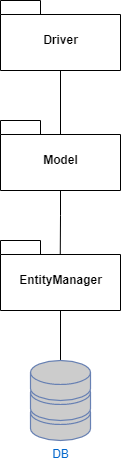
\includegraphics[scale=0.6]{Images/StepImplementation/Step1.png}
    \caption{\textit{Model and Entity Manager} implementation.}
\end{figure}
\subsubsection{Authentication Implementation}
In this step, the components responsible for authentication are implemented and tested, because access to DREAM data and functionalities is a crucial aspect of the system.
\begin{figure}[H]
    \centering
    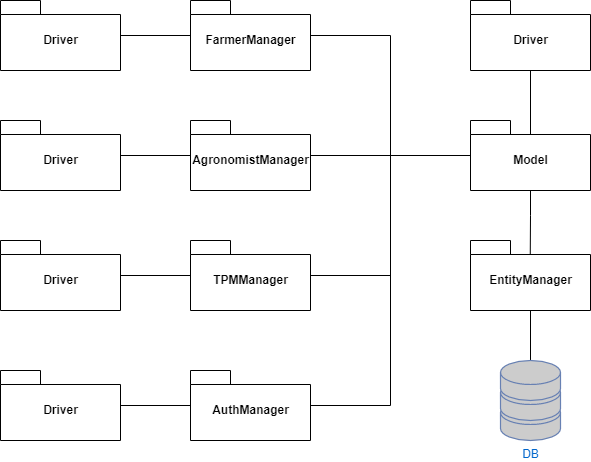
\includegraphics[scale=0.6]{Images/StepImplementation/Step2.png}
    \caption{\textit{Authentication Manager} implementation.}
\end{figure}
\subsubsection{Adding Functionalities}
In this step, the functionalities available in DREAM are implemented one by one. The only functionality that is not yet working is WeatherManager, because it relies on the functioning of the external Forecast Service. While the functionalities dedicated to the production of a farmer are implemented using test data, inserted specifically for the test, since the Sensor Server has not yet been implemented.
\begin{figure}[H]
    \centering
    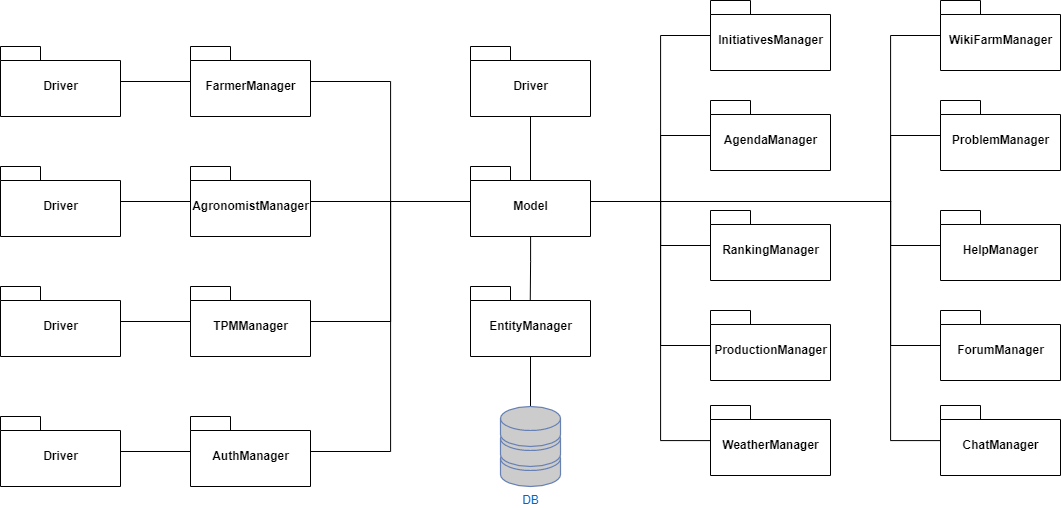
\includegraphics[width=\linewidth]{Images/StepImplementation/Step3.png}
    \caption{\textit{Functionalities} implementation.}
\end{figure}
\subsubsection{Integrating the Forecast Service}
In this step, the WeatherManager functionality is implemented and tested by integrating the functionality with the model and implementing the API provided by the Telangana Weather Service.
\begin{figure}[H]
    \centering
    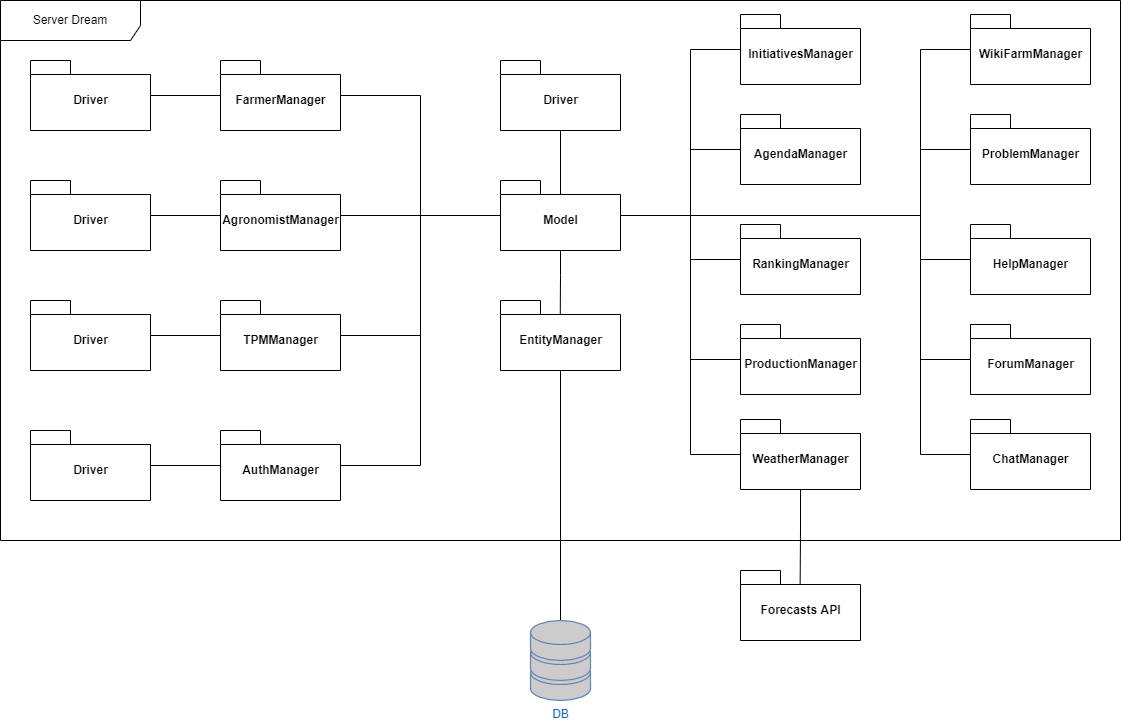
\includegraphics[width=\textwidth]{Images/StepImplementation/Step4.png}
    \caption{\textit{Weather Service} implementation.}
\end{figure}
\newpage
\subsubsection{Testing the Sensor}
The next step is to integrate the server dedicated to managing the Water Usage Sensor and the Humidity Sensor. Before connecting it with the DREAM Server, the operation of the Sensor Server model with sensors is tested.
\begin{figure}[H]
    \centering
    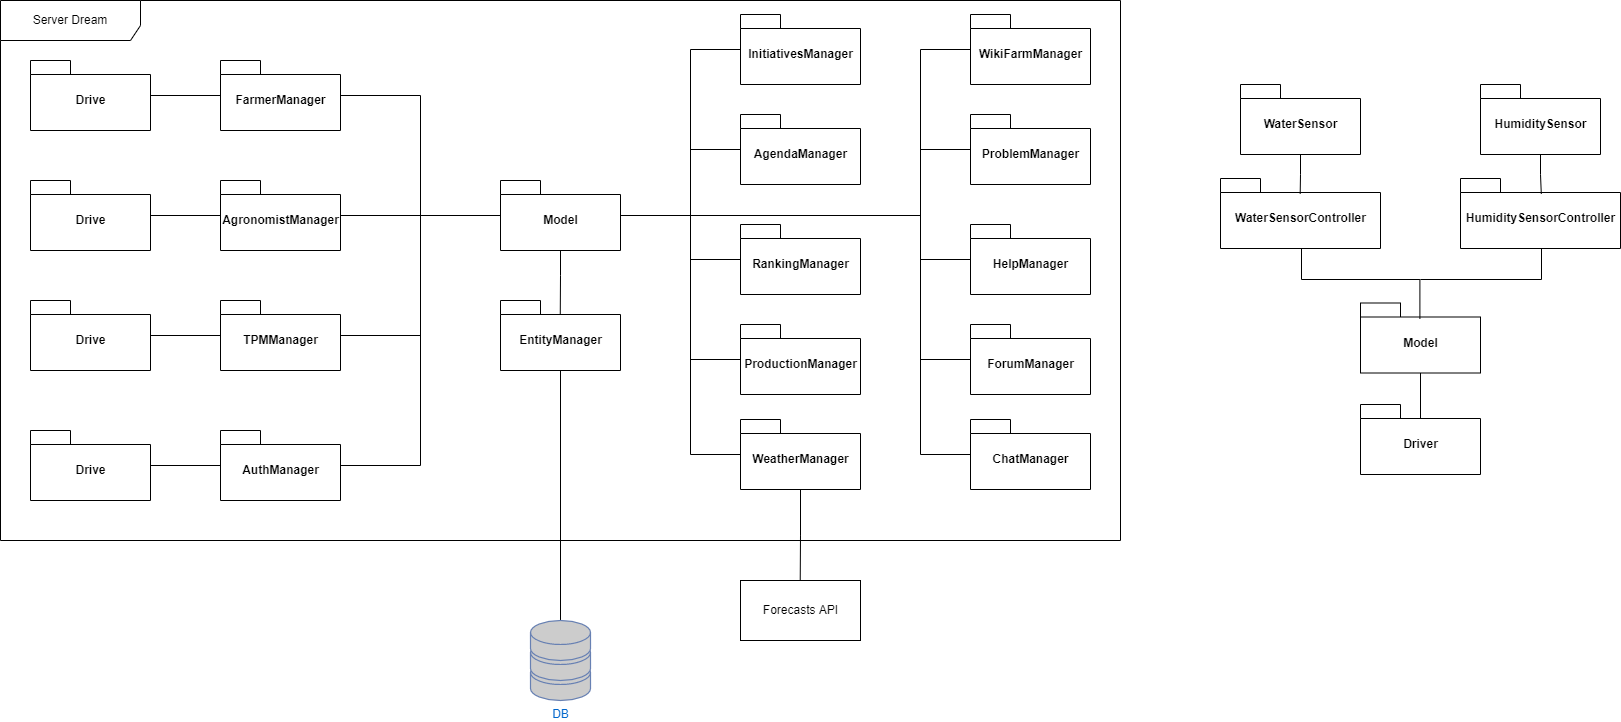
\includegraphics[width=\textwidth]{Images/StepImplementation/Step5.png}
    \caption{\textit{Sensor Server} testing.}
\end{figure}
Once the correct functioning of the Sensor Server has been verified, we proceed to connect it to the Database using the same type of Entity Manager used in the DREAM Server.
\begin{figure}[H]
    \centering
    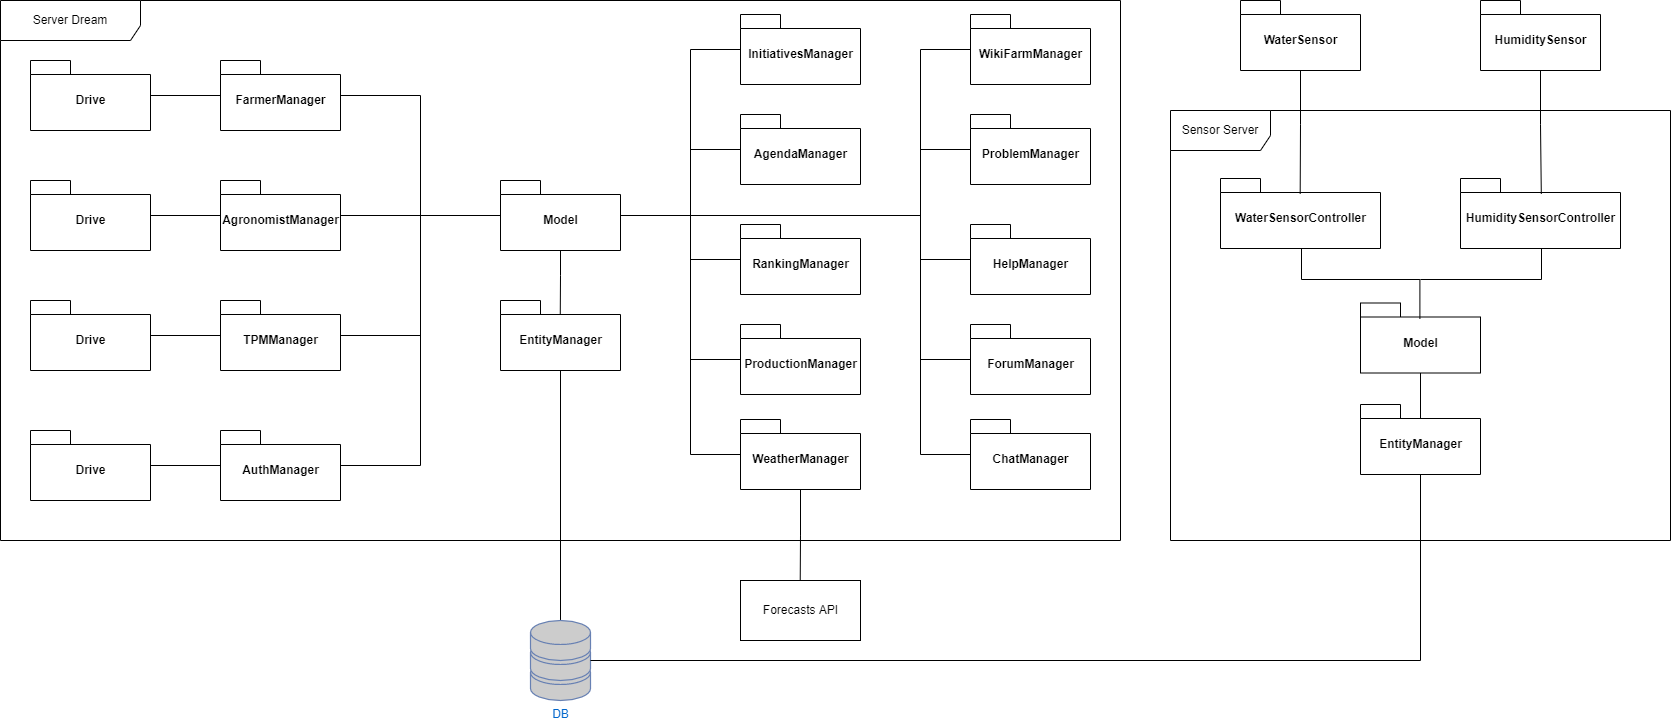
\includegraphics[width=\textwidth]{Images/StepImplementation/Step6.png}
    \caption{\textit{Sensor Server} implementation.}
\end{figure}
\newpage
\subsubsection{Web App Integration}
In this step, the thin client graphics are implemented, and it is checked that all DREAM functions are working properly.
\begin{figure}[H]
    \centering
    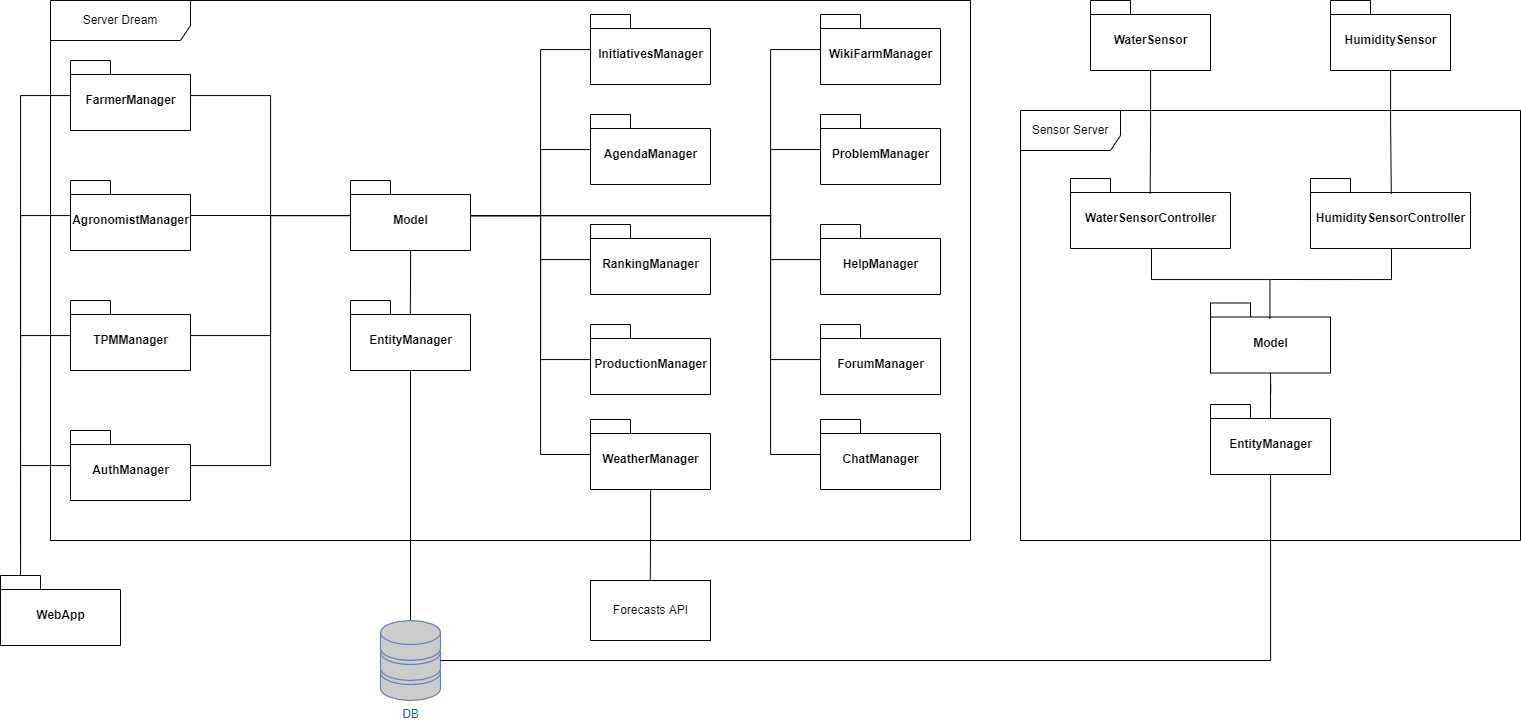
\includegraphics[width=\textwidth]{Images/StepImplementation/Step7.png}
    \caption{\textit{Final} implementation.}
\end{figure}
\newpage
\subsubsection{Final Testing}
Already in the previous step the system was working, but in this step the load balancers are tested and implemented, so as to verify and test the correct functioning of the system at full capacity and with a realistic workload.
\begin{figure}[H]
    \centering
    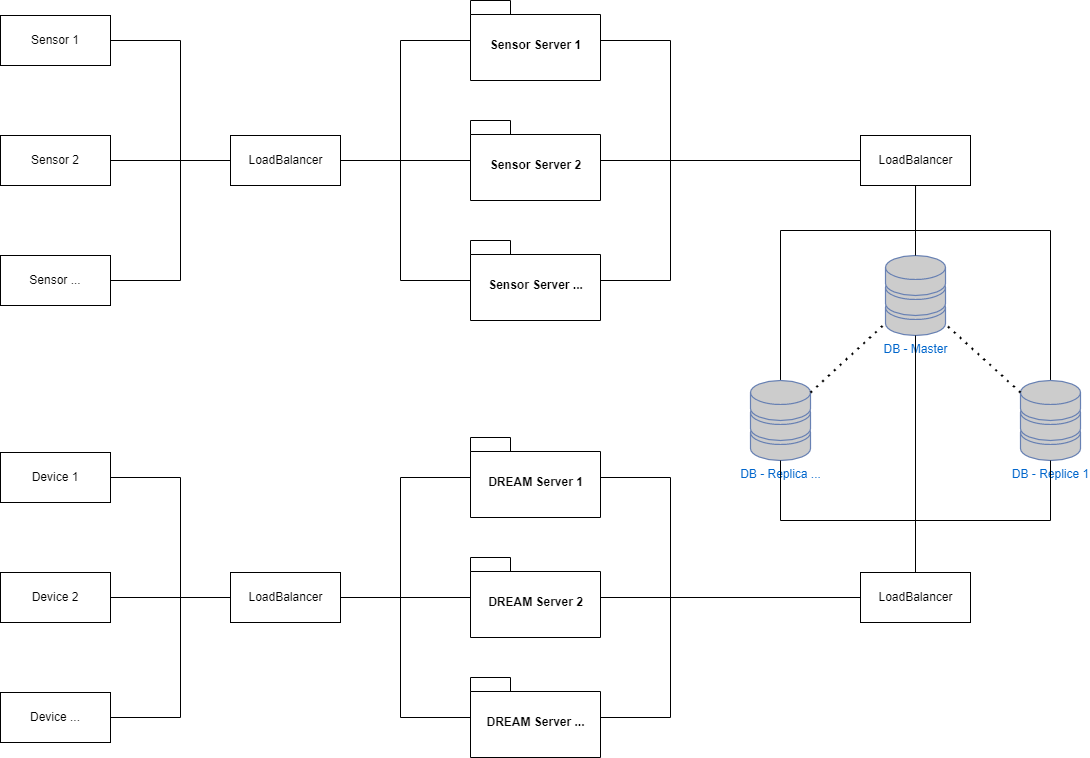
\includegraphics[width=\textwidth]{Images/StepImplementation/Step8.png}
    \caption{\textit{Workload} Testing.}
\end{figure}
\newpage
\subsection{Technologies Used}
This section will analyze the possible technologies available to develop each component of the system.
\subsubsection{Database}
SQLServer was chosen to implement the database because it is one of the most popular and widely used database software in the world, is open source, reliable and easy to keep up to date.
\subsubsection{WebApp}
The WebApp developed must be compatible with all devices and browsers used by the user, which is why it will be implemented using a dynamic page that adapts automatically. For this reason the application will be developed in Java, using Thymeleaf for the template.
\subsubsection{DREAM Server e Sensor Server}
The Sensor Server and DREAM Server will be implemented in Java EE, using TomEE application Web Server. We chose Java EE because it is the most widely used language in server development, is highly supported and offers numerous specially developed APIs. For example, the Java Persistence API (JPA) allows rapid interaction with the database.
\subsubsection{Testing Tool}
Automated tests help ensure that the applications perform correctly before publishing them,
while retaining features and bug fixes velocity. Junit is used for the unit testing framework for the Java programming language. It allows to define the test for each of the parts developed in a Java application. It is very well documented and allows to be integrated with other testing tools.